\subsubsection{Functional Principle}\label{section:license-amazon-functional}
\begin{itemize}
    \item test
\end{itemize}
The prerequesites are the same as with the \gls{lvl}, the developer has to have an account on the Amazon platform.
Amazon has a different approach of implementing the license verification check.
Instead of the developer integrating the license verification library himself, the developer is asked when uploading the application whether it should be integrated (see figure~\ref{fig:amazon}).
According to the description, the library is to \textit{Protect your application from unauthorized use. Without DRM, your app can be used without restrictions by any user.} \cite{amazonDeveloper}
In order to implement the library the \gls{apk} is decompiled server sided, the library is added and the package is then signed with a new signature (see subsection~\ref{subsection:foundation-android-package}).
Amazon describes it as following: \textit{As part of the ingestion process Amazon removes your developer signature and applies an Amazon signature. This signature is unique to you, does not change, and is the same for all apps in your account.} \cite{amazonDeveloper}

 applay amazon DRm to \textit{Protect your application from unauthorized use. Without DRM, your app can be used without restrictions by any user.} as the description says
  as the description says, so developer signing the application by the develoepr before submitting is not necessary, amazon decompiles apk, injects drm code, compiles it and signs it with the \textit{Amazon developer} certificate

when uploading the app, user is asked whether
\begin{figure}[h]
    \centering
    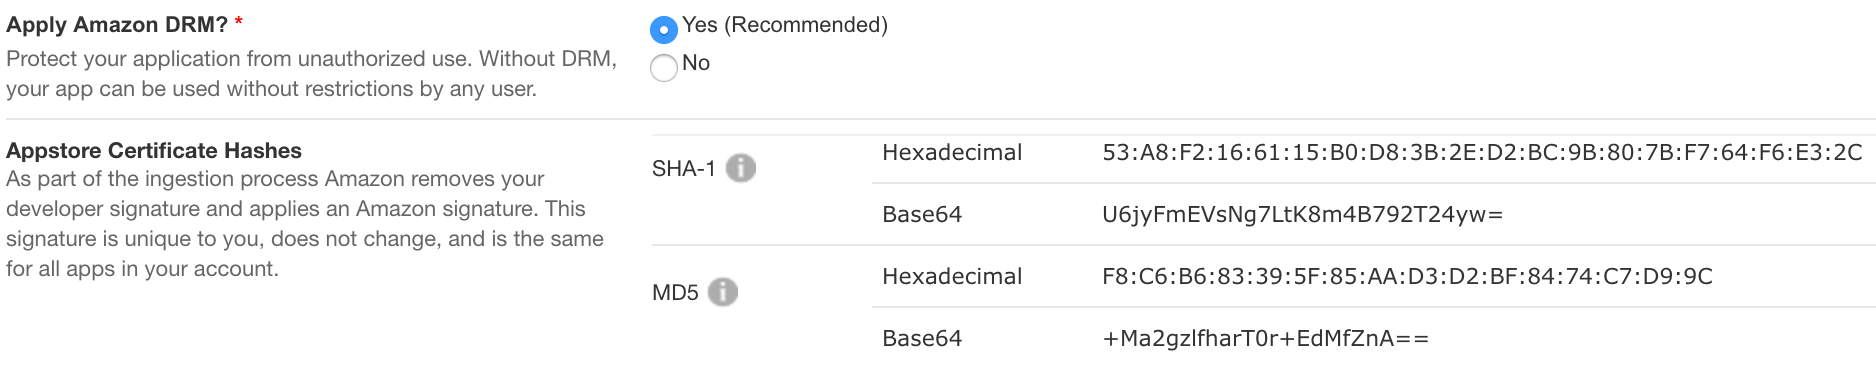
\includegraphics[width=1\textwidth]{data/amazon.png}
    \caption{Developer preferences in the Amazon developer console \cite{amazonDeveloper}}
    \label{fig:amazon}
\end{figure}

%
different approach to perform license verification and enforce result
google lvl include and integrate modified version of lvl library, not required to implement any mechanism on their own, done by amazon packaging tool
when submitting can check amazon DRM (see picture), applay amazon DRm to "Protect your application from unauthorized use. Without DRM, your app can be used without restrictions by any user." as the description says
"As part of the ingestion process Amazon removes your developer signature and applies an Amazon signature. This signature is unique to you, does not change, and is the same for all apps in your account."  as the description says, so developer signing the application by the develoepr before submitting is not necessary, amazon decompiles apk, injects drm code, compiles it and signs it with the "amazon developer" certificate
\cite{munteanLicense}
%




%WAS PASSIERT WENN KEIN PLAYSTORE/AIRPLANE%
amazon appstore has to be installed the whole time and user has to be logged in order that the DRM works

airplane
first time
activity, callback: license not verified
second time
stored license
